\section{Resultados}

O desafio reuniu sete  equipes  de 5 diferentes países, incluindo Brasil, com conhecida expertise em modelagem de dengue para promover um treinamento padronizado de modelos preditivos conjunto (Ensemble) para a dengue no Brasil. Estas equipes enviaram para a plataforma Mosqlimate previsões de dengue usando uma variedade de abordagens de modelagem para as temporadas 2022-2023, 2023-2024 e 2024-2025 para os estados do Amazonas (AM), Ceará (CE), Goiás (GO), Minas Gerais (MG) e Paraná (PR).

Os seguintes resultados foram fornecidos pelos modelos, tanto com estimativas pontuais quanto com intervalos preditivos de 90\%:

 \begin{enumerate}
    \item Curva de casos de dengue por SE para as temporadas de 2023-2024 
    \item Número acumulado de casos prováveis de dengue para UF nas temporadas de 2023-2024
    \item  \end{enumerate}

\subsection{Previsoes de teste para 2023-2024 por UF}

Os gráficos abaixo mostram as curvas epidêmicas previstas e observadas para os dois anos: 2023 e 2024. O código para gerar o gráfico está disponível no \href{https://github.com/Mosqlimate-project/}{Github do projeto Mosqlimate }.

Em 2024, todos os estados apresentaram picos de dengue maiores do que em 2023. Em MG e GO, os picos foram três vezes e cinco vezes maiores, respectivamente. Em geral, o desempenho dos modelos foi melhor em PR e MG, onde todos os modelos previram um aumento no pico epidêmico em 2024. Destacamos o modelo DD como o único que previu aumento em todos os estados, e GHR e KDP como os que tiveram desempenho mais preciso em MG (Figura 1)

\begin{figure}
    \centering
    \includegraphics[width=1\linewidth]{figures/Teste_2023_2024.png}
    \caption{Enter Caption}
    \label{fig:enter-label}
\end{figure}
    

\subsection{Scores dos modelos}

% aqui pode entrar a tabela final do sprint? Apenas ressaltar que nao existe modelo otimo.

\subsection{Previsoes de teste para 2025 por UF}

\begin{figure}
    \centering
    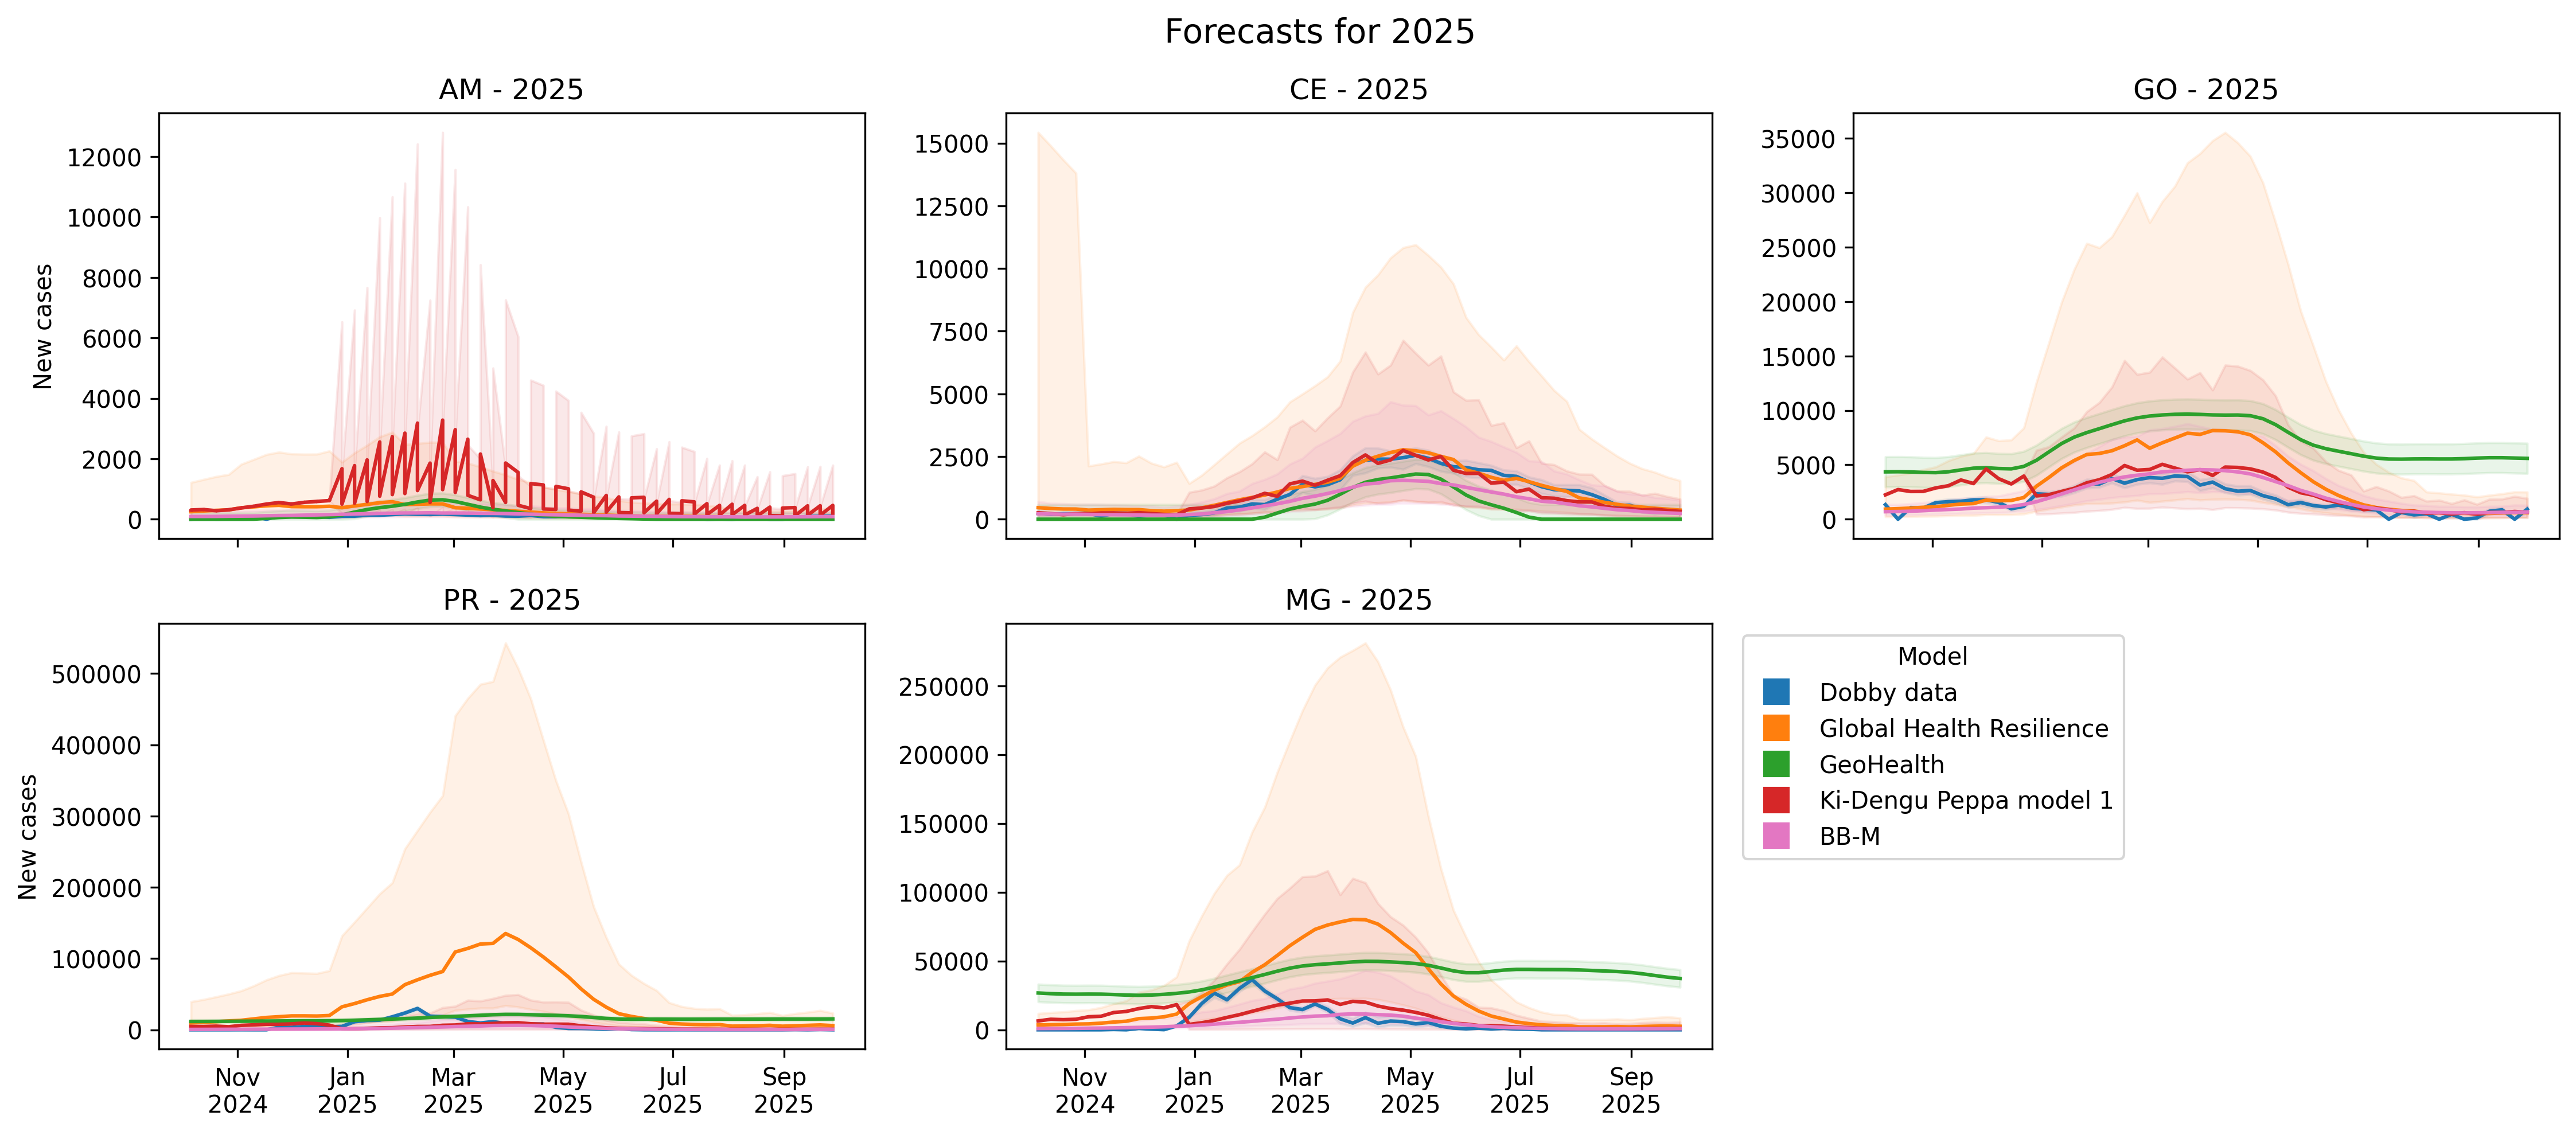
\includegraphics[width=1\linewidth]{figures/forecasts_2025.png}
    \caption{Enter Caption}
    \label{fig:enter-label}
\end{figure}


\subsection{Cenários para 2025, por UF}

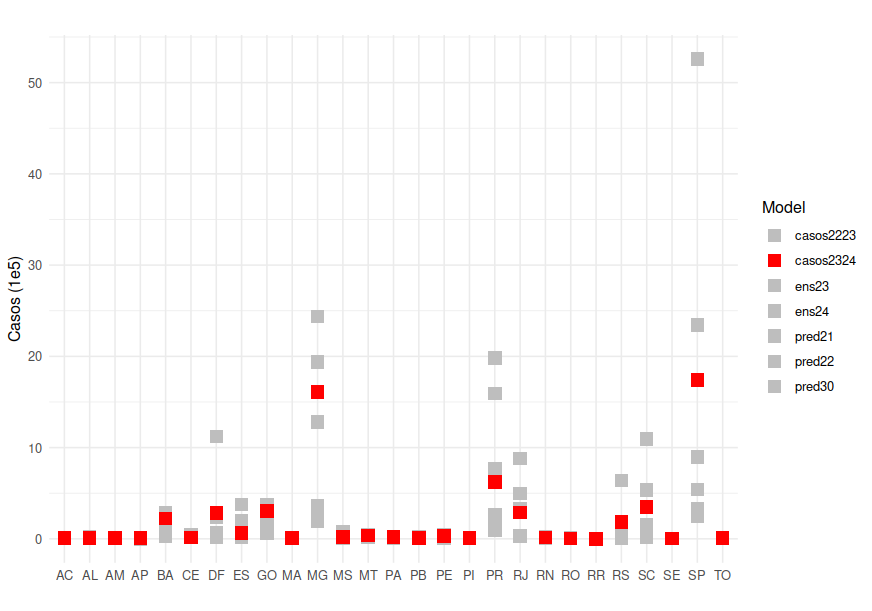
\includegraphics[height = 12cm]{sections/forecast2025.png}

% acrescentar as series dos estados


\subsection{Ensemble 2025 por UF}


\begin{figure}
    \centering
    \includegraphics[width=1\linewidth]{figures/ensemble_stack_final.png}
    \caption{Enter Caption}
    \label{fig:enter-label}
\end{figure}